\documentclass[11pt,spanish,a4paper]{article}
% Versión 2.o cuat 2015 Víctor Bettachini < bettachini@df.uba.ar >

\usepackage{babel}
\addto\shorthandsspanish{\spanishdeactivate{~<>}}
\usepackage[utf8]{inputenc}
\usepackage{float}

\usepackage{units}
\usepackage[separate-uncertainty=true, multi-part-units=single, locale=FR]{siunitx}

\usepackage{amsmath}
\usepackage{amstext}
\usepackage{amssymb}

\newcommand{\pvec}[1]{\vec{#1}\mkern2mu\vphantom{#1}}

\usepackage{tikz}
% \input{DimLinesTikz}
\usetikzlibrary{decorations.pathmorphing, patterns}

\usepackage{graphicx}
\graphicspath{{./graphs/}}

\usepackage[margin=1.3cm,nohead]{geometry}
% \voffset-3.5cm
% \hoffset-3cm
% \setlength{\textwidth}{17.5cm}
% \setlength{\textheight}{27cm}

\usepackage{lastpage}
\usepackage{fancyhdr}
\pagestyle{fancyplain}
\fancyhead{}
\fancyfoot{{\tiny \textcopyright Departamento de Física, FCEyN, UBA}}
\fancyfoot[C]{ {\tiny Actualizado al \today} }
\fancyfoot[RO, LE]{Pág. \thepage/\pageref{LastPage}}
\renewcommand{\headrulewidth}{0pt}
\renewcommand{\footrulewidth}{0pt}

% \def \materia {Física II para químicos}
\def \periodo {cuatrimestre de verano - 2017}
\def \website {http://materias.df.uba.ar/f2qa2017v}


\begin{document}
\noindent
% \textbf{\materia}\hfill \periodo
\textbf{Física II (Químicos)}\hfill \textcopyright {\tt DF, FCEyN, UBA}
\begin{center}
  \textsc{\large Conductores ideales - Capacidad - Conexión de capacitores - Dieléctricos - Capacitor con dieléctricos}  
  % \textsc{\large Guía 2: Conductores ideales - Capacidad - Conexión de capacitores - Dieléctricos - Capacitor con dieléctricos}  
\par\end{center}{\large \par}


\begin{enumerate}
% \begin{description}

\section*{Conductores ideales - Capacidad}

  \item Dentro de un conductor hueco de forma arbitraria, se encuentra alojado un segundo conductor.
  % \item[Problema 1] Dentro de un conductor hueco de forma arbitraria, se encuentra alojado un segundo conductor.
Se carga a uno de ellos con carga \(Q\) y al otro con carga \(Q'\).
¿Sobre cuáles superficies se distribuyen las cargas?
¿Qué ocurre si ambos conductores se tocan?
Muestre que si \(Q'= -Q\), entonces el campo exterior es nulo.
 
 
  \item Un conductor esférico, hueco y sin cargas tiene un radio interior \(a\) y otro exterior \(b\).
  % \item[Problema 2] Un conductor esférico, hueco y sin cargas tiene un radio interior \(a\) y otro exterior \(b\).
En el centro de la esfera se encuentra una carga puntual \(+q\).
¿Cómo es la distribución de cargas?
Calcule y grafique el campo eléctrico y el potencial en todos los puntos del espacio.


  \item En un campo eléctrico uniforme \(\vec{E_0}\) se introduce un cuerpo conductor de forma arbitraria cargado con carga total \(Q\).
  % \item[Problema 3] En un campo eléctrico uniforme \(\vec{E_0}\) se introduce un cuerpo conductor de forma arbitraria cargado con carga total \(Q\).
\begin{enumerate}
  \item ¿Qué valor tiene la fuerza eléctrica que se ejerce sobre el cuerpo?
  \item Como consecuencia de la inducción de cargas sobre la superficie del conductor, el campo dejará de ser uniforme en la vecindad del cuerpo.
Si se ``congela'' la distribución superficial de carga y se quita el campo externo, ¿cómo será el campo en el interior del cuerpo?
Notar que al congelar la carga superficial, el cuerpo pierde las propiedades de un conductor.
\end{enumerate}


  \item Calcular la capacidad de las siguientes configuraciones de conductores:
  % \item[Problema 4] Calcular la capacidad de las siguientes configuraciones de conductores:
\begin{enumerate}
  \item una esfera de radio \(R\) en el vacío; determinar el valor de \(R\) que haga \(C= \SI{1}{\pico\farad}\), 
  \item un condensador esférico de radio interior \(a\) y exterior \(b\) (comparar con el resultado anterior para \(b\) muy grande), 
  \item por unidad de longitud, para un condensador cilíndrico infinito de radios \(R_1\) y \(R_2\),
  \item por unidad de área, para un condensador plano infinito; si la separación entre placas es de \SI{1}{\milli\metre}, dar el valor del área para que \(C =\SI{1}{\farad}\).
\end{enumerate}


\item Una esfera conductora de radio a está rodeada por un casquete esférico, también conductor, de radio interior \(b\) y exterior \(c\).
% \item[Problema 5] Una esfera conductora de radio a está rodeada por un casquete esférico, también conductor, de radio interior \(b\) y exterior \(c\).
Ambos conductores se encuentran unidos por un cable y su carga total es \(Q\).
En el espacio entre ambos se encuentra una superficie esférica de radio \(d\, (a < d < b)\),
cargada con una densidad superficial de carga \(\sigma\).
Calcule el campo eléctrico en todo el espacio (considere que el cable no rompe la simetría esférica del problema). 


\section*{Conexión de capacitores}

\item Un condensador de \SI{1}{\micro\farad} soporta tensiones no mayores de \SI{6}{\kilo\volt}, y otro de \SI{2}{\micro\farad}, no superiores a
% \item[Problema 6] Un condensador de \SI{1}{\micro\farad} soporta tensiones no mayores de \SI{6}{\kilo\volt}, y otro de \SI{2}{\micro\farad}, no superiores a
\SI{4}{\kilo\volt}.
¿Qué tensión soportan si se los conecta en serie?


	\item \begin{minipage}[t]{0.7\textwidth}
		Cuatro capacitores idénticos están conectados a una batería \(V_0\) como se muestra en la figura.
		Al comenzar, la llave 1 está cerrada y la llave 2 está abierta.
		Luego de un tiempo muy largo se abre la llave 1 y se cierra la llave 2.
		¿Cuál será la diferencia de potencial final entre los capacitores si la batería es de \SI{9}{\volt}?
    \end{minipage}
    \begin{minipage}[c][1em][t]{0.25\textwidth}
            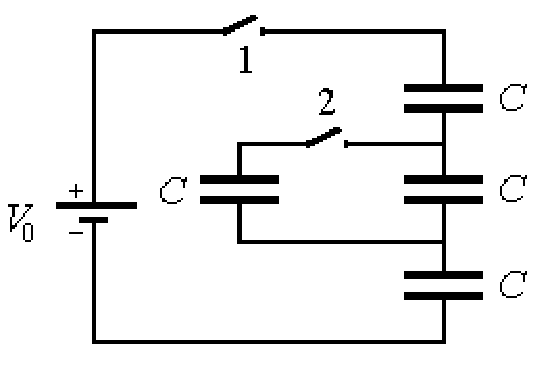
\includegraphics[width=\textwidth]{p2e07}
    \end{minipage}


	\item \begin{minipage}[t]{0.7\textwidth}
		En el circuito de la figura:
		\begin{enumerate}
			\item Calcule la capacidad equivalente que se observa desde la batería.
			\item Encuentre las cargas de cada condensador y calcule la energía del sistema.
			\item Se desconecta la batería. ¿Se redistribuyen las cargas?
			\item Si ahora agregamos un dieléctrico lineal de permitividad \(\varepsilon\) en el condensador \(C_1\) , ¿cómo se redistribuyen las cargas?
				¿Cuál es la energía del sistema?
				¿Dónde está la energía que falta?
		\end{enumerate}
    \end{minipage}
    \begin{minipage}[c][1em][t]{0.25\textwidth}
            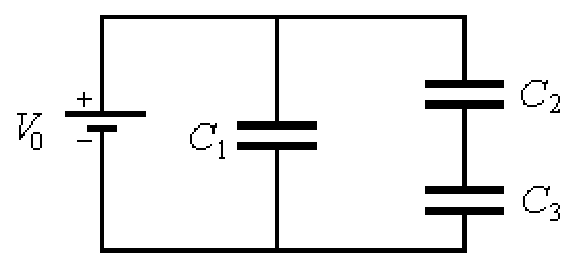
\includegraphics[width=\textwidth]{p2e08}
    \end{minipage}



\section*{Dieléctricos - Capacitor con dieléctricos}

\item Entre las placas de un capacitor plano de sección \(A\) se coloca un dieléctrico como muestra la figura de la izquierda.
% \item[Problema 9] Entre las placas de un capacitor plano de sección \(A\) se coloca un dieléctrico como muestra la figura de la izquierda.
Posteriormente se carga hasta que adquiere una carga \(Q\) y se lo desconecta de la fuente.
\begin{enumerate}
  \item Determine el valor de la capacidad del sistema, la diferencia de potencial entre las placas y la energía acumulada en el capacitor.
  \item ¿Qué sucederá con la carga, la diferencia de potencial y la energía si se le retira el dieléctrico? ¿Y si no se hubiese desconectado la fuente?
  \item Repita los cálculos anteriores para el caso en que el dieléctrico se coloca como muestra la figura de la derecha.
\end{enumerate}
\vspace{-1cm}
\begin{figure}[H]
  \centering{}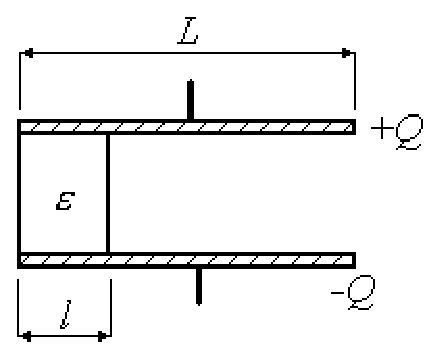
\includegraphics[height= 0.2\textwidth]{p2e09a}
  \centering{}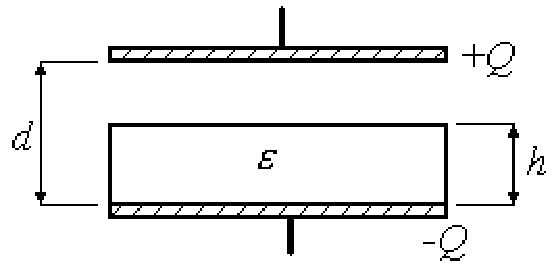
\includegraphics[height= 0.15\textwidth]{p2e09b}
\end{figure}


	\item \begin{minipage}[t][3cm]{0.7\textwidth}
		Entre las placas de un capacitor plano se colocan dos materiales dieléctricos de constantes \(\varepsilon_1\) y \(\varepsilon_2\) como se muestra en la figura.
		Halle la capacidad, considerando que no existen cargas libres en la interfaz entre los dieléctricos.
    \end{minipage}
    \begin{minipage}[c][1em][t]{0.25\textwidth}
            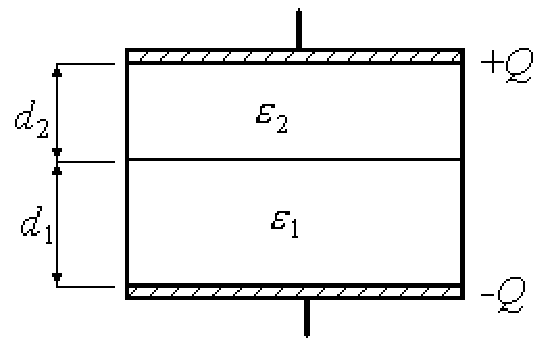
\includegraphics[width=\textwidth]{p2e10}
    \end{minipage}



\item Una esfera cargada uniformemente con carga \(Q\) fue instalada en el seno de un dieléctrico de constante dieléctrica \(\varepsilon\).
% \item[Problema 11] Una esfera cargada uniformemente con carga \(Q\) fue instalada en el seno de un dieléctrico de constante dieléctrica \(\varepsilon\).
Determine la carga de polarización en la interfase entre el dieléctrico y la esfera.



\end{enumerate}
% \end{description}
\end{document}
